\documentclass[a4paper]{article}
\usepackage[affil-it]{authblk}
\usepackage[backend=bibtex,style=numeric]{biblatex}
\usepackage{amsmath, amsthm, amssymb, amsfonts}
\usepackage{graphicx}
\usepackage{multirow}
\usepackage{hyperref}
\usepackage{cleveref}
\hypersetup{
    colorlinks=true,    % 彩色链接
    linkcolor=blue,      % 内部链接的颜色
    citecolor=red,      % 引用的颜色
    urlcolor=cyan       % 外部链接的颜色
}
\usepackage{geometry}
\usepackage[lined, ruled]{algorithm2e}
\geometry{margin=1.5cm, vmargin={0pt,1cm}}
\setlength{\topmargin}{-1cm}
\setlength{\paperheight}{29.7cm}
\setlength{\textheight}{25.3cm}

\crefname{algorithm}{Algorithm}{Algorithms}
\Crefname{algorithm}{Algorithm}{Algorithms}
\crefname{equation}{Equation}{Equations}
\Crefname{equation}{Equation}{Equations}
\crefname{figure}{Figure}{Figures}
\Crefname{figure}{Figure}{Figures}
\crefname{table}{Table}{Tables}
\Crefname{table}{Table}{Tables}

\crefalias{algocf}{algorithm}

\renewcommand\arraystretch{1.8}

\addbibresource{citation.bib}

\begin{document}
% =================================================
\title{\textbf{Numerical Analysis homework \# 2}}

\author{Haowei Peng 3220104816
  \thanks{E-mail address: \texttt{3220104816@zju.edu.cn}}}
\affil{(Information and Computing Science), Zhejiang University} 

\date{Due time: \today}

\maketitle

\begin{abstract}
    The goal of these programming assignments concentrates on the implementation of three numerical methods of solving equations.
    Task A is to design an abstract base class \verb|EquationSolver| and three derived class of it, and use the derived classed to finish the remaining five tasks.
    
    The package \verb|EquationSolver.| contains the implementation details of the \textbf{bisection method, Newton's method and the secant method}, and the series of \verb|Task_X.cpp| finish the task remaining.
    By using the package I design, the equations can be solved by calling the corresponding method of the \verb|EquationSolver| class.

    In this report, I will introduce the design of the package and the algorithms used in the it. 
    And I'll give the result of the tasks. 
    Especially, I use the \textbf{function pointer} instead of a base class of function.
\end{abstract}

% ============================================
\section*{A.\ Design a Class of EquationSolver}

\subsection*{A.1\ Algorithms Used in the Package}

\subsubsection*{A.1.1\ Bisection Method}

The bisection method is a root-finding algorithm that applied to continuous functions. It is a simple and effective method to find a root of a function. 

The algorithm starts with an interval $[a, b]$ and repeatedly bisect the interval until the desired root is bracketed by two values $c_1$ and $c_2$ such that $f(c_1)f(c_2) < 0$. The root is then approximated as the average of $c_1$ and $c_2$. 
And it terminates when the width of the interval is smaller than a given tolerance $\delta$ or when a maximum number of iterations $M$ is reached.

The specific algorithm is given below:

\begin{algorithm}[H]
  \KwIn{$f: [a,\ b] \rightarrow \mathbb{R},\ a \in \mathbb{R},\ b \in \mathbb{R},\ M \in \mathbb{N},\ \delta \in \mathbb{R}^+,\ \varepsilon \in \mathbb{R}^+ $}
  \SetKw{Require}{Preconditions: }
  \Require{$f \in \mathcal{C}[a,\ b],\ \mathrm{sgn}(f(a)) \ne \mathrm{sgn}(f(b))$}\\
  \KwOut{$c,\ h,\ k$}
  \SetKw{Ensure}{Postconditions: }
  \Ensure{$|f(c)| < \varepsilon \ \mathrm{or} \ |h| < \delta \ \mathrm{or} \ k = M$}\\
  \BlankLine
  \LinesNumbered
  $h \leftarrow b - a$\;
  $u \leftarrow f(a)$\;
  \For{$k = 0:M$}{
    $h \leftarrow h/2$\;
    $c \leftarrow a + h$\;
    \uIf{$|w| < \varepsilon$}{
      \textbf{break}
    }
    \ElseIf{$\mathrm{sgn}(w) = \mathrm{sgn}(u)$}{
      $a \leftarrow c$\;
    }
  }
  \caption{Bisection Method}
  \label{al:Bisection_method}
\end{algorithm}

\subsubsection*{A.1.2\ Newton's Method}

The Newton's method is a more accurate method for finding root. It is based on the Taylor series expansion of the function and needs the function be $\mathcal{C}^2$.

The iteration formula is given by:
\begin{equation}
  x_{n + 1} = x_n - \frac{f(x_n)}{f'(x_n)}, \quad n \in \mathbb{N}
  \label{eq:Newton_method}
\end{equation}

\begin{algorithm}[H]
  \KwIn{$f: \mathbb{R} \rightarrow \mathbb{R},\ f',\ x_0 \in \mathbb{R},\ M \in \mathbb{N}^+,\ \varepsilon \in \mathbb{R}^+$}
  \SetKw{Require}{Preconditions: }
  \Require{$f \in \mathcal{C}^2$ and $x_0$ is sufficiently close to a root of $f$}\\
  \KwOut{$x,\ k$}
  \SetKw{Ensure}{Postconditions: }
  \Ensure{$|f(x)| < \varepsilon \ \mathrm{or} \ k = M$}\\
  \BlankLine
  \LinesNumbered
  $x \leftarrow x_0$\;
  \For{$k = 0:M$}{
    $u \leftarrow f(x)$\;
    \If{$|u| < \varepsilon$}{
      \textbf{break}
    }
    $x \leftarrow x - u/f'(x)$\;
  }
  \caption{Newton's method}
  \label{al:Newton_method}
\end{algorithm}

It can be proved that the Newton's method converges at least quadratically to the root $\alpha$ of the function.

\subsubsection*{A.1.3\ Secant Method}

The secant method is based on the tangent line to the curve $f(x)$ at the points $x_0$ and $x_1$. The iteration formula can be conveyed as follows:
\begin{equation}
  x_{n + 1} = x_n - f(x_n) \cdot \frac{x_n - x_{n - 1}}{f(x_n) - f(x_{n - 1})}, \quad n \in \mathbb{N}
  \label{eq:Secant_method}
\end{equation}

\begin{algorithm}[H]
  \KwIn{$f: \mathbb{R} \rightarrow \mathbb{R},\ x_0,\ x_1 \in \mathbb{R},\ M \in \mathbb{N}^+,\ \delta \in \mathbb{R}^+,\ \varepsilon \in \mathbb{R}^+$}
  \SetKw{Require}{Preconditions: }
  \Require{$f \in \mathcal{C}^2,\ x_0,\ x_1$ are sufficiently close to a root of $f$}\\
  \KwOut{$k,\ x_n,\ n_{n - 1}$}
  \SetKw{Ensure}{Postconditions: }
  \Ensure{$|f(x_n)| < \varepsilon \ \mathrm{or} \ |x_n - x_{n-1}| < \delta \ \mathrm{or} \ k = M$}\\
  \BlankLine
  \LinesNumbered
  $x_n \leftarrow x_1$\;
  $x_{n-1} \leftarrow x_0$\;
  $u \leftarrow f(x_n)$\;
  $v \leftarrow f(x_{n-1})$\;
  \For{$k = 1:M$}{
    $s \leftarrow \frac{x_n - x_{n-1}}{u - v}$\;
    $x_{n - 1} \leftarrow x_n$\;
    $v \leftarrow u$\;
    $x_n \leftarrow x_n - u \cdot s$\;
    \If{$|x_n - x_{n - 1}| < \delta$}{
      \textbf{break}
    }
    $u \leftarrow f(x_n)$\;
    \If{$|u| < \varepsilon$}{
      \textbf{break}
    }
  }
  \caption{Secant method}
  \label{al:Secant_method}
\end{algorithm}

It can be proved that the secant method converges to the root $\alpha$ with order $p = \frac{1}{2}(1 + \sqrt{5}) \approx 1.618$.

\subsection*{A.2\ Design of the Package}

\subsubsection*{A.2.1\ EquationSolver Class}

The \verb|EquationSolver| class is an abstract base class that contains the common interface for all three numerical methods. 
It contains two protected member \verb|equation_| and \verb|derivative_|, which are the equation and its derivative, respectively. 

The function \verb|solve| is a pure virtual function with parameters \verb|tol_func, tol_x, a, b|, where 
\begin{enumerate}
  \item \verb|tol_func|: the tolerance of the function value, i.e. $\varepsilon$ in the algorithms;
  \item \verb|tol_x|: the tolerance of the root, i.e. $\delta$ in the algorithms;
  \item \verb|a|: the lower bound of the interval or the initial guess of the root;
  \item \verb|b|: the upper bound of the interval or the initial guess of the root.
\end{enumerate}

\subsubsection*{A.2.2\ Three Derived Classes}

The three derived classes are \verb|Bisection_Method, Newton_Method, Secant_Method|, which implement the corresponding algorithms mentioned in \cref{al:Bisection_method,al:Newton_method,al:Secant_method}.

In general, I use the \textbf{function pointer} to implement the algorithms. The function pointer is a pointer to a function that can be assigned to a variable. 
Especially, I set a judgement condition in the \verb|Bisection_Method| class to determine whether the precondition is met.

\section*{B. Test My Implementation of the Bisection Method}

\subsection*{B.1\ Problem Statement}

The functions and intervals are given as follows:
\begin{itemize}
  \item $x^{-1} - \tan x \ \mathrm{on} \ [0,\ \pi/2]$
  \item $x^{-1} - 2^x \ \mathrm{on} \ [0,\ 1]$
  \item $2^{-x} + e^x + 2 \cos x - 6 \ \mathrm{on} \ [1,\ 3]$
  \item $(x^3 + 4x^2 + 3x + 5)/(2x^3 - 9x^2 + 18x - 2) \ \mathrm{on} \ [0,\ 4]$
\end{itemize}

\subsection*{B.2\ Results of the Bisection Method}

The first three tasks' results are shown in \cref{tab:B.1-B.3} as follows.

\begin{table}[htbp]
  \centering
  \begin{tabular}{|c|c|c|}
    \hline 
    \textbf{Function and Interval} & \textbf{Root} & \textbf{Error} \\
    \hline
    $x^{-1} - \tan x \ \mathrm{on} \ [0,\ \pi/2]$ & 0.86026453 & 0.00025565 \\
    \hline
    $x^{-1} - 2^x \ \mathrm{on} \ [0,\ 1]$ & 0.64113159 & 0.00019027 \\
    \hline 
    $2^{-x} + e^x + 2 \cos x - 6 \ \mathrm{on} \ [1,\ 3]$ & 1.82940674 & 0.00009490 \\
    \hline
  \end{tabular}
  \caption{Results of Task B.1 - B.3}
  \label{tab:B.1-B.3}
\end{table}

For the task of solving $(x^3 + 4x^2 + 3x + 5)/(2x^3 - 9x^2 + 18x - 2) \ \mathrm{on} \ [0,\ 4]$, 
we can know that $x^3 + 4x^2 + 3x + 5 > 0$ on $[0,\ 4]$, so the root does not exist on this interval. The image of the function is shown below \cref{fig:task_b4}.

\begin{figure}[htbp]
  \centering
  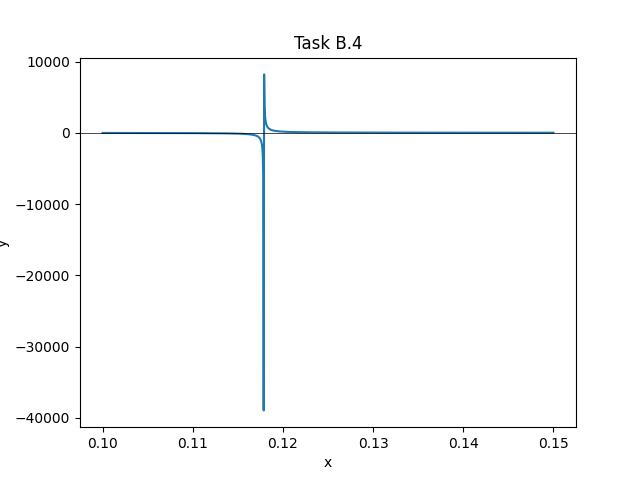
\includegraphics[width = 0.6\textwidth]{../images/task_b4.png}
  \caption{The image of the function on $[0.10,\ 0.15]$}
  \label{fig:task_b4}
\end{figure}

Through the \cref{al:Bisection_method}, we can know that the bisection method is to approach a region where the function value changes sign. 
So for this task, the bisection method will find the root of $2x^3 - 9x^2 + 18x - 2$ on $[0,\ 4]$.

\begin{table}[htbp]
  \centering
  \begin{tabular}{|c|c|c|}
    \hline 
    \textbf{Function and Interval} & \textbf{Root} & \textbf{Error} \\
    \hline
    $(x^3 + 4x^2 + 3x + 5)/(2x^3 - 9x^2 + 18x - 2) \ \mathrm{on} \ [0,\ 4]$ & 0.11785986 & 20286.88841693 \\
    \hline
  \end{tabular}
  \caption{Results of Task B.4}
  \label{tab:B.4}
\end{table}

Let $x = 0.11785986$, $2x^3 - 9x^2 + 18x - 2 = -0.00026667$.

\section*{C.\ Test My Implementation of the Newton's Method}

\subsection*{C.1\ Problem Statement}

The problem asks us to solve the equation $x = \tan x$ and find the roots near 4.5 and 7.7 respectively.

\subsection*{C.2\ Results of the Newton's Method}

The results of the Newton's method are shown as follows:
\begin{table}[htbp]
  \centering
  \begin{tabular}{|c|c|c|}
    \hline 
    \textbf{The Initial Guess} & \textbf{Root} & \textbf{Error} \\
    \hline
    4.5 & 4.49340946 & 0.00000000 \\
    \hline
    7.7 & 7.72525184 & 0.00000000 \\ 
    \hline
  \end{tabular}
  \caption{Results of Task C}
  \label{tab:C}
\end{table}

\section*{D.\ Test My Implementation of the Secant Method}

\subsection*{D.1\ Problem Statement}

The assignment needs us to solve the functions following with the given initial values:
\begin{itemize}
  \item $\sin (x/2) - 1$
  \begin{itemize}
    \item $x_0 = 0,\ x_1 = \frac{\pi}{2}$
    \item $x_0 = \frac{7\pi}{2},\ x_2 = 4\pi$
  \end{itemize}
  \item $e^x - \tan x$
  \begin{itemize}
    \item $x_0 = 1,\ x_1 = 1.4$
    \item $x_0 = -3,\ x_1 = -3.4$
  \end{itemize}
  \item $x^3 - 12x^2 + 3x + 1$
  \begin{itemize}
    \item $x_0 = 0,\ x_1 = -0.5$
    \item $x_0 = 0,\ x_1 = 0.5$
  \end{itemize}
\end{itemize}

\subsection*{D.2\ Results of the Secant Method}

The results of the Secant method are shown as follows:

\begin{table}[htbp]
  \centering
  \begin{tabular}{|c|c|c|c|}
    \hline 
    \textbf{Function} & \textbf{Initial Values} & \textbf{Root} & \textbf{Error} \\
    \hline
    \multirow{2}{*}{$\sin \frac{x}{2} - 1$} & $x_0 = 1,\ x_1 = \frac{\pi}{2}$ & 3.13879506 & 0.00000098 \\
    \cline{2-4}
    & $x_0 = \frac{7\pi}{2},\ x_1 = 4\pi$ & 15.70602631 & 0.00000047 \\
    \hline
    \multirow{2}{*}{$e^x - \tan x$} & $x_0 = 1,\ x_1 = 1.4$ & 1.30632693 & 0.00000017 \\
    \cline{2-4}
    & $x_0 = -3,\ x_1 = -3.4$ & -3.09641230 & 0.00000000 \\
    \hline
    \multirow{2}{*}{$x^3 - 12x^2 + 3x + 1$} & $x_0 = 0,\ x_1 = -0.5$ & -0.18868540 & 0.00000001 \\
    \cline{2-4}
    & $x_0 = 0,\ x_1 = 0.5$ & 0.45154321 & 0.00000011 \\
    \hline
  \end{tabular}
  \caption{Results of Task D}
  \label{tab:D}
\end{table}

\section*{E.\ Use the Three Implementations to Solve the Parameter of a Trough}

\subsection*{E.1\ Problem Statement}

As shown in \cref{fig:E}, a trough of length $L$ has a cross section in the shape of a semi-circle with radius $r$. 
When filled to within a distance $h$ of the top, the water has the volume 
\begin{equation}
  V = L\left[ 0.5\pi r^2 - r^2 \arcsin \frac{h}{r} - h(r^2 - h^2)^{\frac{1}{2}} \right].
  \label{eq:E.V} 
\end{equation}
where $L = 10\ \text{ft},\ r = 1\ \text{ft}, V = 12.4\ \text{ft}^3$.

\begin{figure}[htbp]
  \centering
  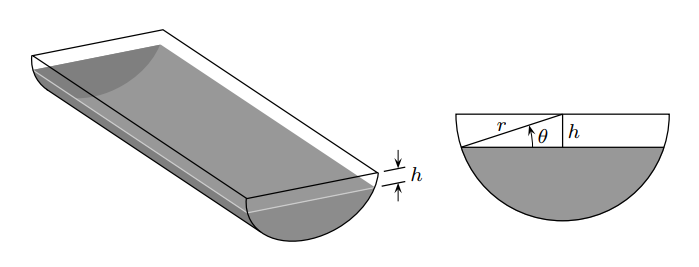
\includegraphics[width = 0.4\textwidth]{../images/E.png}
  \caption{a trough of length $L$}
  \label{fig:E}
\end{figure}

The task is to find the depth of water in the trough to within $0.01$ ft by each of the three implementations in assignment A, and the depth of water is
\begin{equation}
  d = r - h
  \label{eq:E.d}
\end{equation}
where $h$ is the root of the \cref{eq:E.V}.

\subsection*{E.2\ Results}

The results of the three implementations are shown as follows:
\begin{table}[htbp]
  \centering
  \begin{tabular}{|c|c|c|c|}
    \hline
    \textbf{Method} & \textbf{Root} $h$ & \textbf{Depth of Water} $d$ & \textbf{Error} \\
    \hline
    Bisection Method & 0.16 & 0.84 & 0.04 \\
    \hline 
    Newton's Method & 0.17 & 0.83 & 0.00 \\
    \hline 
    Secant Method & 0.17 & 0.83 & 0.00 \\
    \hline
  \end{tabular}
  \caption{Results of Task E}
\end{table}

\section*{F. Use the Three Implementations to Solve the Angle of a Vehicle}

\subsection*{F.1\ Problem Statement}

In the design of all-terrain vehicles, we need to consider the \textit{hang-up failure} and \textit{nose-in failure}. 
The following \cref{fig:F} shows the components associated with the nose-in failure of a vehicle. 

\begin{figure}[htbp]
  \centering
  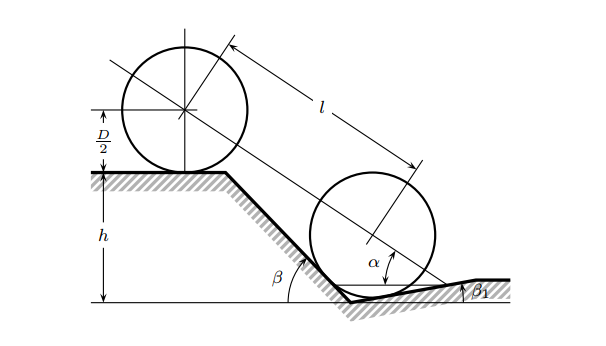
\includegraphics[width = 0.4\textwidth]{../images/F.png}
  \caption{an all-terrain vehicle with nose-in failure}
  \label{fig:F}
\end{figure}

In this problem, it satisfies the equation
\begin{equation}
  A \sin \alpha \cos \alpha + B \sin^2 \alpha - C \cos \alpha - E \sin \alpha = 0
  \label{eq:F}
\end{equation}
where $\alpha$ is the maximum angle and $\beta$ is the maximum angle at which hang-up failure doesn't occur, and 
\begin{equation}
  \begin{aligned}
    A &= l \sin \beta_1,\ B = l \cos \beta_1, \\
    C &= (h + 0.5D)\sin \beta_1 - 0.5 D \tan \beta_1, \\
    E &= (h + 0.5D)\cos \beta_1 - 0.5D.
  \end{aligned}
  \label{eq:F.components}
\end{equation}

The problem is divided into three parts:
\begin{enumerate}
  \item Use Newton's method to verify $\alpha \approx 33^{\circ}$ when $l = 89\ \mathrm{in.},\ h = 49\ \mathrm{in.},\ D = 55\ \mathrm{in.},$ and $\beta_1 = 11.5^{\circ}$.
  \item Use Newton's method with the initial guess $33^{\circ}$ with $D = 30\ \mathrm{in.}$.
  \item Use the secant method (with another initial value as far away as possible from $33^{\circ}$) to find $\alpha$.
\end{enumerate}

\subsection*{F.2\ Results}

The results of the task are shown as follows:
\begin{table}[htbp]
  \centering
  \begin{tabular}{|c|c|c|c|c|}
    \hline
    & \textbf{Initial Guess} & \textbf{Root} & \textbf{$\alpha$} & \textbf{Error} \\
    \hline 
    (a) & $x_0 = 33^{\circ}$ & 0.57547301 & $32.97217470^{\circ}$ & 0.00000000 \\
    \hline 
    (b) & $x_0 = 33^{\circ}$ & 0.57890658 & $33.16890377^{\circ}$ & 0.00000000 \\
    \hline 
    \multirow{3}{*}{(c)} & $x_0 = 33^{\circ} ,\ x_1 = 93^{\circ}$ & 0.57547301 & $32.97217470^{\circ}$ & 0.00000000 \\
    \cline{2-5}
    & $x_0 = 33^{\circ} ,\ x_1 = 153^{\circ}$ & 0.57547314 & $32.97218215^{\circ}$ & 0.00000687 \\
    \cline{2-5}
    & $x_0 = 33^{\circ} ,\ x_1 = 348.5^{\circ}$ & 6.08247244 & $348.50000000^{\circ}$ & 0.00000000 \\
    \hline
  \end{tabular}
  \caption{Results of Task F}
  \label{tab:F}
\end{table}

\subsection*{F.3\ Explanation of Task F(c)}

From the case (c) of \cref{tab:F}, we can see that we will get a different result if the initial value is too far away from $33^{\circ}$. 
Firstly we should mention that the trigonometric functions are periodic, so the root of the function will be periodic as well. 
According to \cref{eq:Secant_method} and the result of (a), we can know that $\alpha \approx 33^{\circ}$ is extremely close to the accurate root of the equation. 

By plugging \cref{eq:F.components} into \cref{eq:F}, we can simplify the equation as follows:
\begin{equation}
    (l\sin \alpha - h - 0.5D + \frac{0.5D}{\cos \beta_1}) \sin (\alpha + \beta_1) = 0
    \label{eq:F.re}
\end{equation}

Consequently, the task F(c) has the analytical solution 
\begin{equation}
  \alpha = -\beta_1
  \label{eq:F.sol}
\end{equation}

The \cref{eq:F.sol} above can explain the another result of \cref{eq:F}.

% ===============================================
\section*{ \center{\normalsize {Acknowledgement}} }
In the process of finishing the task, I get help from the \href{https://kimi.moonshot.cn}{\textit{Kimi AI}} and the extension named \href{https://code.fittentech.com/tutor_vscode_en}{\textit{Fitten Code}} in the VSCode in these aspects:
\begin{enumerate}
  \item How to insert a function into a package;
  \item How to debug some grammar errors in C++;
  \item How to write some things in \TeX. 
\end{enumerate}

And I check the official documents of some packages of \TeX \ such as \textit{algorithm2e}, \textit{cleveref} and so on.

Besides, I use 3.14159265358979323846 to approximate $\pi$ in these tasks.

For the task F(c), I exchange the ideas with Yuqing Yan. He firstly get a root $x = -11.5^{\circ}$, and then I get the analytical solution $\alpha = -\beta_1$.

\printbibliography

\end{document}